\documentclass[11pt,a4paper]{article}
\usepackage[utf8]{inputenc}
\usepackage[T1]{fontenc}
\usepackage[francais]{babel}
\usepackage{amsmath}
\usepackage{amsfonts}
\usepackage{amssymb}
\usepackage{graphicx}
\usepackage{fullpage}
\usepackage{tikz}
\usepackage{algorithm}
\usepackage{algpseudocode}
\usepackage{enumitem}

\title{Algo avancée \\ Travailler moins pour manger plus}

\newcommand{\second}{\prime\prime}

\begin{document}
	\maketitle
	\section{Énoncé}
	
\includegraphics[width=0.99\textwidth]{Algo-tmpmp.jpg}
	
	\section{Formalisation}
	
	\begin{itemize}
		\item n champs $1 \leqslant j \leqslant n$
		\item $s_j$ : surface du champs j
		\item $t_j$ : type du champs j
		\item n produits \begin{align*}
							\Rightarrow 1 \leqslant &i \leqslant n\\
							\Rightarrow 1 \leqslant &i_j \leqslant n\\
							\Rightarrow &\text{permutations}\\
							&\begin{cases}
								1 \leqslant j \leqslant n\\
								\ \ \ \ \ \ \ \updownarrow\\
								1 \leqslant i_j \leqslant n\\
							\end{cases}
						 \end{align*}
		\item S est une permutation de $[1,n] = {i_1, i_2, i_3, ..., i_n}$
	\end{itemize}
	Notre critère d'évaluation : le travail w
	$$v(s)= \sum_{j=1}^{n} s_j w_{i_{j},t_{j}}$$
	
	\section{Résolution séparation et évaluation}
	
	Le niveau k permet de choisir $i_k$. Chaque feuille est une solution.
	$$v(S_k) \rightarrow \underset{\hookrightarrow\text{évaluation}}{e(S_k)} = \sum_{j=1}^{n} s_j w_{i_{j},t_{j}}$$
	
	
	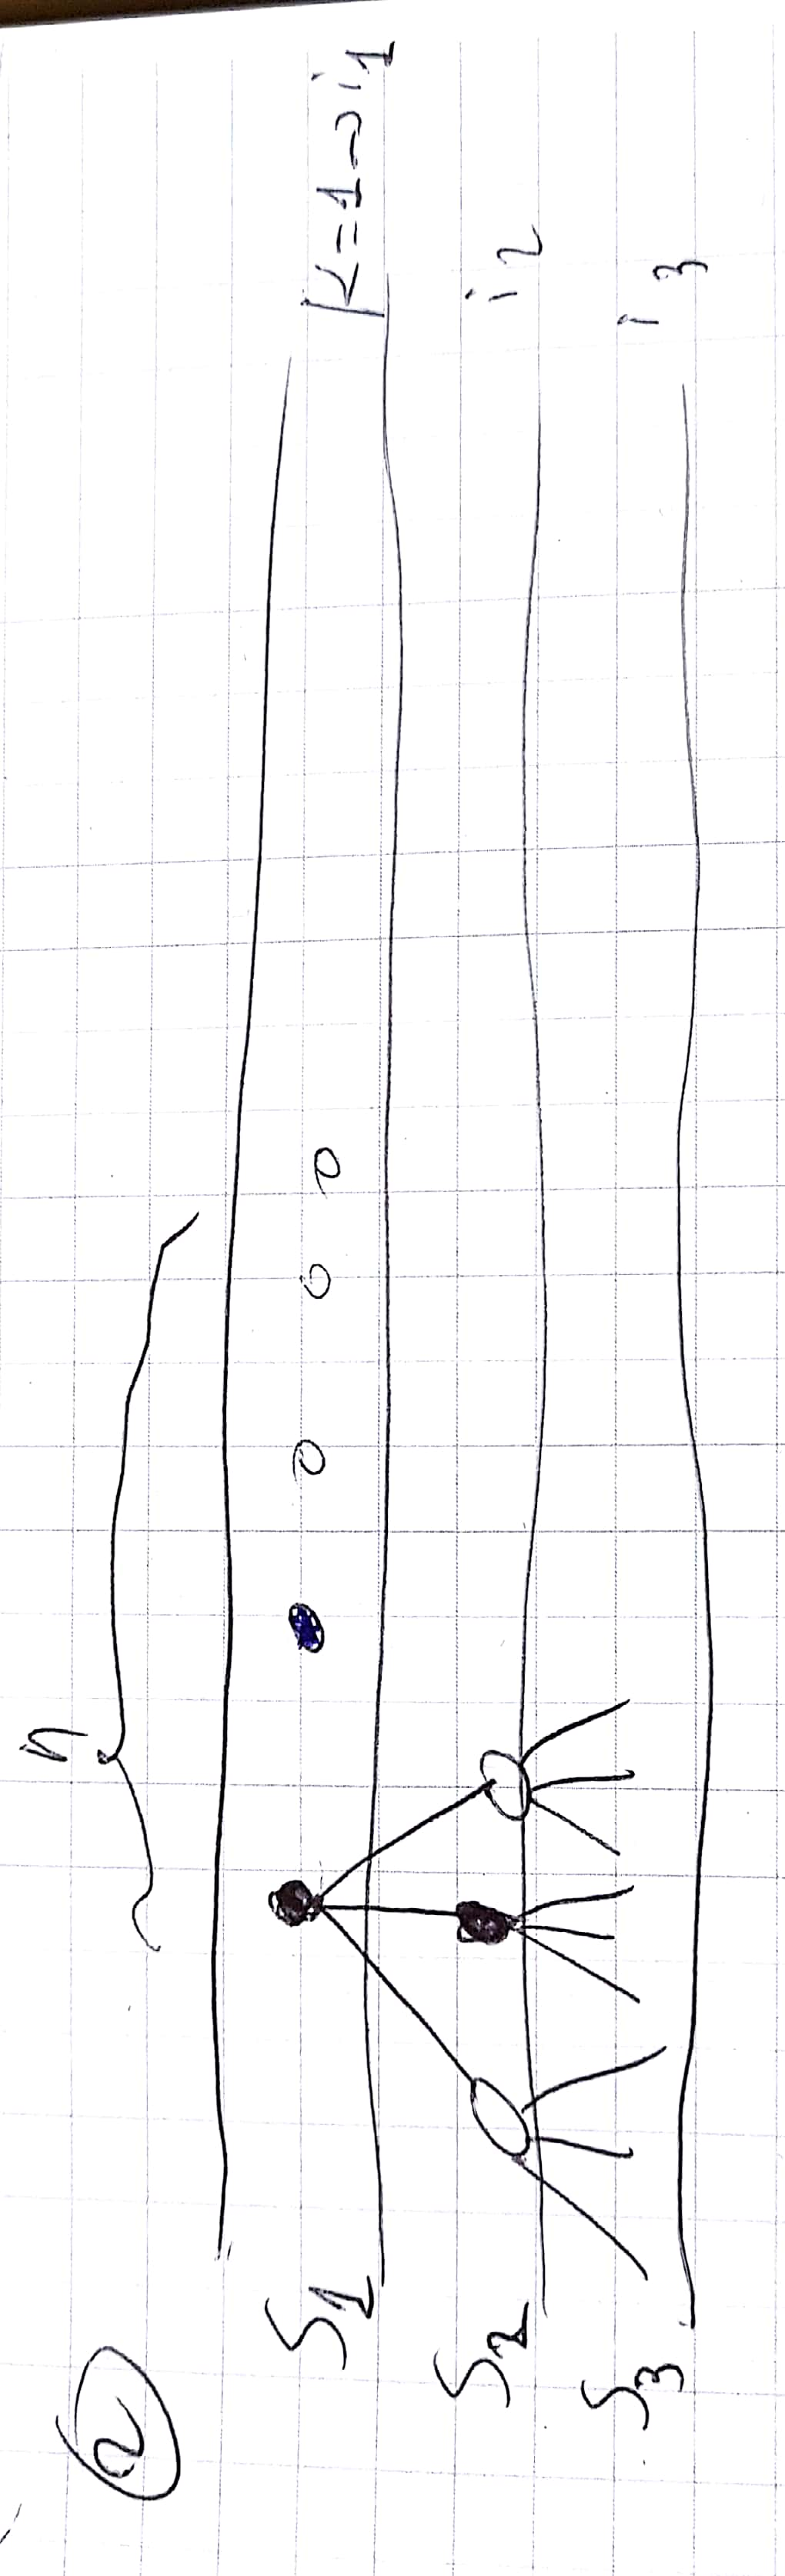
\includegraphics[angle=-90,width=0.99\textwidth]{schema.jpg}
	
	Au noeud k, $e(S_k)$ est plus petit que toutes les feuilles du sous arbre $\leftarrow$ critère de séparation.
	
	$$e^\prime(S_k) = e(S_k) + \sum_{j=k+1}^{n} s_j\ min(w_{i_{j},t_{j}})$$
	(Reste un minorant des feuilles du sous-arbre)
	$$e^{\second} = e(S_k) + \sum_{j=k+1}^{n} s_j\ \underset{i_j \notin S_k}{min(w_{i_{j},t_{j}})}$$
	
	
\end{document}